% Presentazione: dalle equazioni complete alle equazioni frazionarie.
% Si compila con XeLaTeX (come gli appunti):
%   latexmk -xelatex -outdir=build appunti-matematica-3b-equazioni-frazionarie.tex
% Immagini e crediti in immagini-frazionarie/.
\documentclass[aspectratio=169,11pt]{beamer}

\usepackage{fontspec}
\setmainfont{TeX Gyre Pagella}
\setsansfont{TeX Gyre Heros}
\usepackage{polyglossia}
\setmainlanguage{italian}
\usepackage{amsmath,amssymb,mathtools}
\usepackage{unicode-math}
\setmathfont{TeX Gyre Pagella Math}
\usefonttheme{serif}

\usepackage{tikz}
\usetikzlibrary{arrows.meta,positioning}
\usepackage{pgfplots}
\pgfplotsset{compat=1.18}
\usepackage{booktabs}

% Colori
\definecolor{blu}{HTML}{1D4ED8}
\definecolor{rosso}{HTML}{DC2626}
\definecolor{oro}{HTML}{B7791F}
\definecolor{verde}{HTML}{15803D}
\definecolor{grigio}{HTML}{64748B}
\definecolor{seme}{HTML}{8A5A12}
\setbeamercolor{frametitle}{fg=blu}
\setbeamercolor{title}{fg=blu}
\setbeamercolor{structure}{fg=blu}
\setbeamercolor{block title}{fg=white,bg=blu}
\setbeamercolor{block body}{bg=blu!6}
\setbeamercolor{block title alerted}{fg=white,bg=rosso}
\setbeamercolor{block body alerted}{bg=rosso!6}
\setbeamertemplate{navigation symbols}{}
\setbeamertemplate{footline}{\hfill\textcolor{grigio}{\footnotesize\insertframenumber}\hspace{1em}\vspace{0.6em}}

% Oggetti TikZ/pgfplots che compaiono solo da una certa slide in poi
\tikzset{
  invisible/.style={opacity=0},
  visible on/.style={alt={#1{}{invisible}}},
  alt/.code args={<#1>#2#3}{\alt<#1>{\pgfkeysalso{#2}}{\pgfkeysalso{#3}}},
  nota/.style={font=\itshape, text=rosso},
}

\newcommand{\virgola}{{,}}
\newcommand{\aureo}{\textcolor{oro}{\varphi}}
% riga di tabella che compare dalla slide #1 in poi
\newcommand{\riga}[4]{\uncover<#1->{#2} & \uncover<#1->{#3} & \uncover<#1->{#4}}

% Crescita di un girasole (modello di Vogel). Nasce un seme alla volta, sempre
% al centro; ogni seme nuovo è ruotato rispetto al precedente di #2 giri.
% I semi più vecchi vengono spinti verso l'esterno: dopo #1 semi, il seme i
% sta a distanza #3·√(#1−i+1) dal centro.
% #1 = semi nati finora, #2 = rotazione in frazioni di giro
% (0.381966 = 1/φ² ≈ 137,5°; 0.25 = 90°; 0.4 = 144°), #3 = scala, #4 = raggio del seme
\newcommand{\crescita}[4]{%
  \foreach \i in {1,...,#1}{%
    \pgfmathsetmacro{\giri}{\i*#2}%
    \fill[seme] ({360*(\giri-floor(\giri))}:{#3*sqrt(#1-\i+1)}) circle[radius=#4];
  }%
}
% Come sopra, per pochi semi: ogni seme porta il suo numero, l'ultimo nato è rosso.
% I semi si possono richiamare come nodi s1, s2, ...
\newcommand{\crescitanum}[3]{%
  \foreach \i in {1,...,#1}{%
    \pgfmathsetmacro{\giri}{\i*#2}%
    \ifnum\i=#1 \def\col{rosso}\else\def\col{seme}\fi
    \node[circle, fill=\col, text=white, inner sep=0pt, minimum size=4.5mm, font=\scriptsize\bfseries]
      (s\i) at ({360*(\giri-floor(\giri))}:{#3*sqrt(#1-\i+1)}) {\i};
  }%
}

\title{Dividere per $x$}
\subtitle{Dalle equazioni di secondo grado alle equazioni frazionarie}
\author{Prof.\ Fulvio Bergadano}
\institute{Liceo Vittoria}
\date{}

\begin{document}

\begin{frame}
  \titlepage
\end{frame}

% ============================================================
% La risolvo alla lavagna, scrivendo sulla proiezione.
\begin{frame}{Un'equazione che sappiamo risolvere}
  \[
    x^2 = x + 1
  \]
  \vfill
  \pause
  \[
    x_{1,2} = \frac{1 \pm \sqrt5}{2}
    \qquad
    x_1 \approx 1\virgola618 \qquad x_2 \approx -0\virgola618
  \]
\end{frame}

\begin{frame}{Un'altra strada: divido per $x$}
  \[
    x^2 = x + 1
  \]
  \pause
  \[
    \frac{x^2}{x} = \frac{x+1}{x}
  \]
  \pause
  \begin{center}
    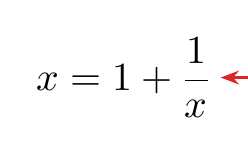
\begin{tikzpicture}
      \node[font=\Large] (eq) {$\displaystyle x = 1 + \frac1x$};
      \node[draw=rosso, rounded corners, text=rosso, font=\large, right=1.5cm of eq,
            overlay, visible on=<4->] (ric) {ricorsione};
      \draw[-{Stealth}, rosso, thick, overlay, visible on=<4->] (ric) -- (eq);
    \end{tikzpicture}
  \end{center}
\end{frame}

\begin{frame}{Un castello di frazioni}
  \[
    x = 1 + \frac{1}{\textcolor{rosso}{x}}
  \]
  \vspace{0.5em}
  \only<2>{\[
    x = 1 + \cfrac{1}{\textcolor{rosso}{1 + \cfrac{1}{x}}}
  \]}%
  \only<3>{\[
    x = 1 + \cfrac{1}{1 + \cfrac{1}{\textcolor{rosso}{1 + \cfrac{1}{x}}}}
  \]}%
  \only<4>{\[
    x = 1 + \cfrac{1}{1 + \cfrac{1}{1 + \cfrac{1}{1+\cfrac{1}{1+\cfrac{1}{\;\ddots\;}}}}}
  \]}
\end{frame}

\begin{frame}{Costruiamo il castello piano per piano}
  \begin{columns}[T]
    \begin{column}{0.4\textwidth}
      \centering
      \begin{tabular}{ccc}
        \toprule
        piano & frazione & valore \\
        \midrule
        1  & $1$ & $1$ \\
        \riga{2}{2}{$2$}{$2$} \\
        \riga{3}{3}{$3/2$}{$1\virgola5$} \\
        \riga{4}{4}{$5/3$}{$1\virgola6667$} \\
        \riga{5}{5}{$8/5$}{$1\virgola6$} \\
        \riga{6}{6}{$13/8$}{$1\virgola625$} \\
        \riga{7}{7}{$21/13$}{$1\virgola6154$} \\
        \riga{8}{8}{$34/21$}{$1\virgola6190$} \\
        \riga{9}{9}{$55/34$}{$1\virgola6176$} \\
        \riga{10}{10}{$89/55$}{$1\virgola6182$} \\
        \riga{11}{11}{$144/89$}{$1\virgola6180$} \\
        \bottomrule
      \end{tabular}
    \end{column}
    \begin{column}{0.58\textwidth}
      \centering
      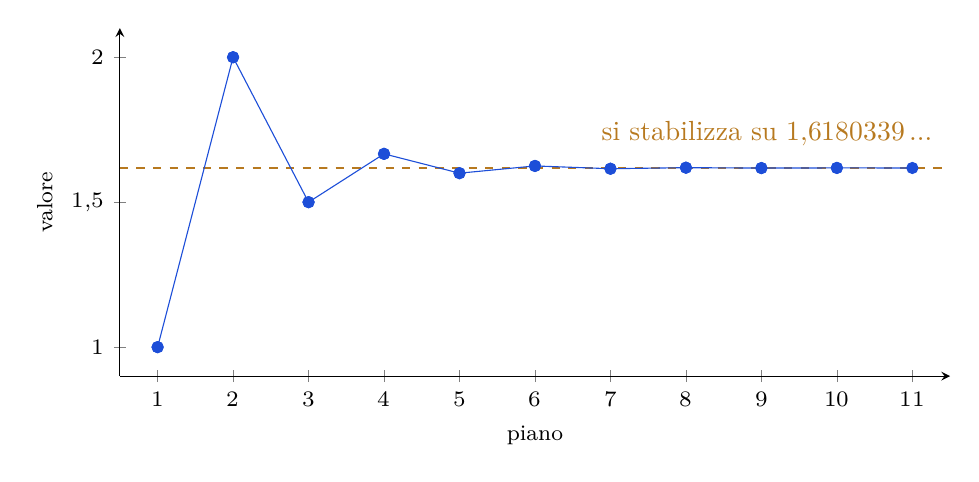
\begin{tikzpicture}
        \begin{axis}[
          width=\linewidth, height=6cm,
          xmin=0.5, xmax=11.5, ymin=0.9, ymax=2.1,
          xtick={1,...,11}, ytick={1,1.5,2},
          yticklabels={$1$,$1\virgola5$,$2$},
          xlabel={piano}, ylabel={valore},
          tick label style={font=\footnotesize},
          label style={font=\footnotesize},
          axis lines=left,
        ]
          \addplot[oro, dashed, thick, domain=0.5:11.5, visible on=<12->] {1.6180339887};
          \addplot[blu, thin, mark=*, mark size=2pt, visible on=<1->]  coordinates {(1,1)};
          \addplot[blu, thin, mark=*, mark size=2pt, visible on=<2->]  coordinates {(1,1)(2,2)};
          \addplot[blu, thin, mark=*, mark size=2pt, visible on=<3->]  coordinates {(2,2)(3,1.5)};
          \addplot[blu, thin, mark=*, mark size=2pt, visible on=<4->]  coordinates {(3,1.5)(4,1.66667)};
          \addplot[blu, thin, mark=*, mark size=2pt, visible on=<5->]  coordinates {(4,1.66667)(5,1.6)};
          \addplot[blu, thin, mark=*, mark size=2pt, visible on=<6->]  coordinates {(5,1.6)(6,1.625)};
          \addplot[blu, thin, mark=*, mark size=2pt, visible on=<7->]  coordinates {(6,1.625)(7,1.61538)};
          \addplot[blu, thin, mark=*, mark size=2pt, visible on=<8->]  coordinates {(7,1.61538)(8,1.61905)};
          \addplot[blu, thin, mark=*, mark size=2pt, visible on=<9->]  coordinates {(8,1.61905)(9,1.61765)};
          \addplot[blu, thin, mark=*, mark size=2pt, visible on=<10->] coordinates {(9,1.61765)(10,1.61818)};
          \addplot[blu, thin, mark=*, mark size=2pt, visible on=<11->] coordinates {(10,1.61818)(11,1.61798)};
          \node[oro, anchor=south east, visible on=<12->] at (axis cs:11.4,1.66) {si stabilizza su $1\virgola6180339\ldots$};
        \end{axis}
      \end{tikzpicture}
    \end{column}
  \end{columns}
\end{frame}

\begin{frame}{Che numero è?}
  \[
    1\virgola6180339\ldots \;=\; \frac{1+\sqrt5}{2} \;=\; \aureo
    \qquad \text{la \textbf{sezione aurea}}
  \]
  \pause
  \vspace{1em}
  \[
    \frac{\textcolor{blu}{1}}{1},\ \frac{\textcolor{blu}{2}}{1},\ \frac{\textcolor{blu}{3}}{2},\
    \frac{\textcolor{blu}{5}}{3},\ \frac{\textcolor{blu}{8}}{5},\ \frac{\textcolor{blu}{13}}{8},\
    \frac{\textcolor{blu}{21}}{13},\ \ldots
    \qquad\longrightarrow\qquad
    \textcolor{blu}{1,\ 1,\ 2,\ 3,\ 5,\ 8,\ 13,\ 21,\ \ldots}
  \]
  \pause
  \begin{center}
    numeri di \textbf{Fibonacci}: ognuno è la somma dei due precedenti
  \end{center}
\end{frame}

% ============================================================
% L'altra radice: con un'altra ricorsione diventa lei il punto d'arrivo.
\begin{frame}{E la soluzione negativa?}
  \pause
  Riconsideriamo la nostra equazione $x^2=x+1$ \pause e raccogliamo $x$:
  \[
    x^2 - x = 1
    \quad\Rightarrow\quad
    x\,(x-1) = 1
  \]
  \pause
  Dividiamo per $x-1$:
  \[
    x = \frac{1}{-1+x}
    \qquad\pause \textcolor{rosso}{\text{un'altra ricorsione}}
  \]
  \pause
  \[
    x = \cfrac{1}{-1 + \cfrac{1}{-1 + \textcolor{rosso}x}}
  \]
  \pause
  \[
    0 \;\to\; -1 \;\uncover<4->{\to\; -0\virgola5} \;\uncover<5->{\to\; -0\virgola667}
    \;\uncover<6->{\to\; -0\virgola6} \;\uncover<7->{\to\; -0\virgola625} \;\uncover<8->{\to\; -0\virgola615 \;\to\;\cdots}
  \]
  \uncover<9->{\[
    \boxed{\;x_2 = \frac{1-\sqrt5}{2} \approx -0\virgola618\;}
  \]}
\end{frame}

% ============================================================
\begin{frame}
  \centering
  \Large\textcolor{oro}{Intermezzo}\\[0.5em]
  \huge La sezione aurea in natura
\end{frame}

% Quadrati di Fibonacci accostati: a ogni passo il rettangolo totale ha per lati
% due numeri di Fibonacci consecutivi, quindi il rapporto dei lati tende a φ.
\begin{frame}{Il rettangolo aureo}
  \centering
  \begin{tikzpicture}[scale=0.3, line width=0.5pt]
    \path (-3,-5) rectangle (22,16); % riquadro fisso: la figura non salta fra le slide
    \draw[fill=blu!10]  (0,0) rectangle (1,1);
    \draw<2->[fill=blu!15] (1,0) rectangle (2,1);
    \draw<3->[fill=blu!20] (0,1) rectangle (2,3);
    \node<3->[font=\scriptsize] at (1,2) {2};
    \draw<4->[fill=blu!25] (-3,0) rectangle (0,3);
    \node<4->[font=\footnotesize] at (-1.5,1.5) {3};
    \draw<5->[fill=blu!30] (-3,-5) rectangle (2,0);
    \node<5->[font=\small] at (-0.5,-2.5) {5};
    \draw<6->[fill=blu!35] (2,-5) rectangle (10,3);
    \node<6->[font=\normalsize] at (6,-1) {8};
    \draw<7->[fill=blu!40] (-3,3) rectangle (10,16);
    \node<7->[font=\large] at (3.5,9.5) {13};
    % rapporto fra i lati del rettangolo, scritto a fianco
    \node[anchor=west, font=\large] at (12,6) {%
      \only<1>{$\dfrac11 = 1$}\only<2>{$\dfrac21 = 2$}\only<3>{$\dfrac32 = 1\virgola5$}%
      \only<4>{$\dfrac53 \approx 1\virgola667$}\only<5>{$\dfrac85 = 1\virgola6$}%
      \only<6>{$\dfrac{13}{8} \approx 1\virgola625$}%
      \only<7->{$\dfrac{21}{13} \approx 1\virgola615 \approx \aureo$}};
    % spirale: un quarto di cerchio in ogni quadrato
    \begin{scope}[oro, line width=1.8pt, visible on=<8->]
      \draw (0,1)   arc[start angle=180, end angle=270, radius=1];
      \draw (1,0)   arc[start angle=270, end angle=360, radius=1];
      \draw (2,1)   arc[start angle=0,   end angle=90,  radius=2];
      \draw (0,3)   arc[start angle=90,  end angle=180, radius=3];
      \draw (-3,0)  arc[start angle=180, end angle=270, radius=5];
      \draw (2,-5)  arc[start angle=270, end angle=360, radius=8];
      \draw (10,3)  arc[start angle=0,   end angle=90,  radius=13];
    \end{scope}
    \node[oro, anchor=west, font=\large\itshape, visible on=<8->] at (12,2) {spirale aurea};
  \end{tikzpicture}
\end{frame}

% Il girasole, come cartone animato. Regola: i semi nascono uno alla volta al
% centro, e ogni seme nuovo nasce ruotato di 137,5° rispetto al precedente.
% Crescendo, i vecchi vengono spinti fuori. Il numero aureo è nell'angolo:
% 137,5° e 222,5° dividono il giro in sezione aurea (222,5/137,5 = 360/222,5 = φ).
\begin{frame}{Come cresce un girasole}
  \begin{columns}[c]
    \begin{column}{0.36\textwidth}
      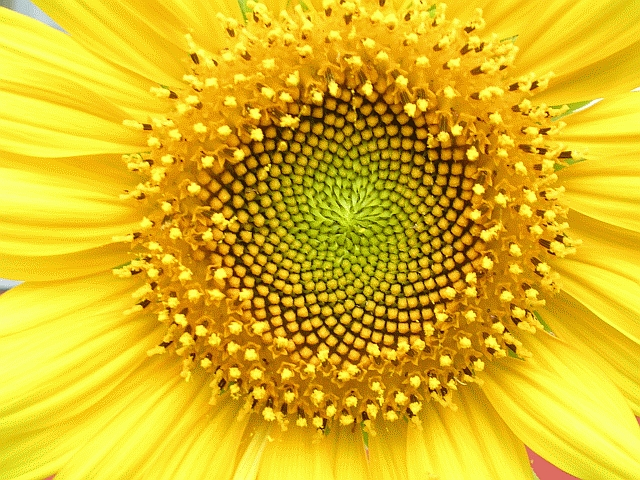
\includegraphics[width=\linewidth]{immagini-frazionarie/girasole.jpg}
    \end{column}
    \begin{column}{0.62\textwidth}
      \centering
      \begin{tikzpicture}[scale=0.95]
        \path (-3.3,-3.3) rectangle (3.3,3.3);
        % il centro del girasole, sempre segnato
        \draw[gray, thick] (-0.15,0) -- (0.15,0) (0,-0.15) -- (0,0.15);
        \only<1>{\crescitanum{1}{0.381966}{1.2}
          \node[nota, right=3mm of s1] {nasce il 1° seme};
          \node[nota, text=gray, anchor=north] at (0,-0.25) {centro};}
        \only<2>{\crescitanum{2}{0.381966}{1.2}
          \draw[gray, dashed] (0,0) -- (s1); \draw[gray, dashed] (0,0) -- (s2);
          \draw[-{Stealth}, rosso, thick] (137.5:0.75) arc[start angle=137.5, end angle=275, radius=0.75];
          \node[nota, anchor=north east] at (215:1.0) {ruota di $137\virgola5^\circ$};}
        \only<3>{\crescitanum{3}{0.381966}{1.2}
          \draw[gray, dashed] (0,0) -- (s2); \draw[gray, dashed] (0,0) -- (s3);
          \draw[-{Stealth}, rosso, thick] (275:0.75) arc[start angle=275, end angle=412.5, radius=0.75];
          \node[nota, anchor=west] at (345:1.05) {ancora $137\virgola5^\circ$};}
        \only<4>{\crescitanum{4}{0.381966}{1.2}
          \draw[gray, dashed] (0,0) -- (s3); \draw[gray, dashed] (0,0) -- (s4);
          \draw[-{Stealth}, rosso, thick] (52.5:0.75) arc[start angle=52.5, end angle=190, radius=0.75];
          \node[nota] at (0,-2.9) {i semi vecchi vengono spinti fuori};}
        \only<5>{\crescitanum{6}{0.381966}{1.2}}
        \only<6>{\crescitanum{10}{0.381966}{1.2}}
        \only<7>{\crescita{30}{0.381966}{0.55}{0.1}}
        \only<8>{\crescita{80}{0.381966}{0.36}{0.085}}
        \only<9>{\crescita{200}{0.381966}{0.23}{0.07}}
        \only<10>{\crescita{500}{0.381966}{0.145}{0.055}}
      \end{tikzpicture}
    \end{column}
  \end{columns}
\end{frame}

\begin{frame}{Dov'è il numero aureo?}
  \centering
  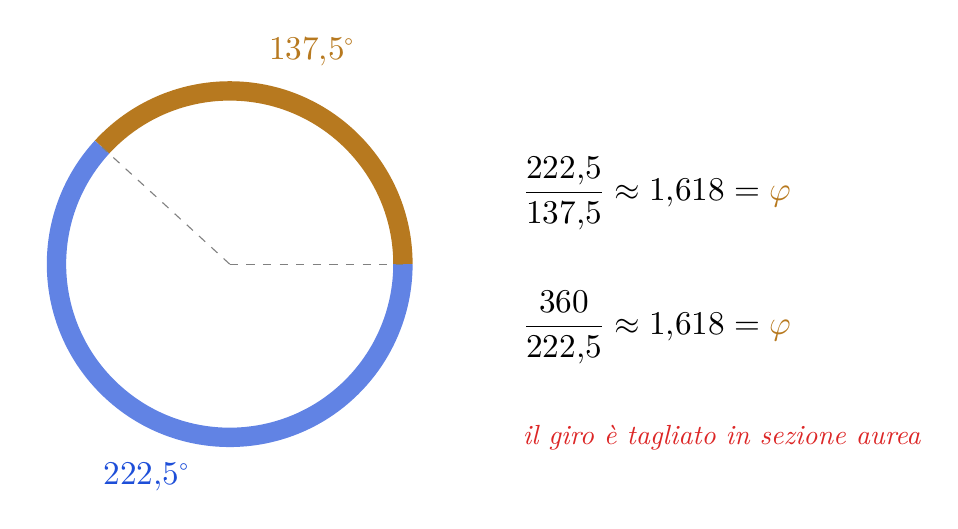
\begin{tikzpicture}
    \draw[line width=7pt, oro]  (0:2.2) arc[start angle=0, end angle=137.5, radius=2.2];
    \draw[line width=7pt, blu!70] (137.5:2.2) arc[start angle=137.5, end angle=360, radius=2.2];
    \draw[gray, dashed] (0,0) -- (0:2.2); \draw[gray, dashed] (0,0) -- (137.5:2.2);
    \node[oro, font=\large] at (68.75:2.9) {$137\virgola5^\circ$};
    \node[blu, font=\large] at (248.75:2.9) {$222\virgola5^\circ$};
    \node[font=\large, anchor=west] at (3.6,0.9) {$\dfrac{222\virgola5}{137\virgola5} \approx 1\virgola618 = \aureo$};
    \node[font=\large, anchor=west, visible on=<2->] at (3.6,-0.8) {$\dfrac{360}{222\virgola5} \approx 1\virgola618 = \aureo$};
    \node[nota, anchor=west, visible on=<3->] at (3.6,-2.2) {il giro è tagliato in sezione aurea};
  \end{tikzpicture}
\end{frame}

% Perché proprio quell'angolo. Con 1/4 di giro il 5° seme nasce nella stessa
% direzione del 1°, il 6° del 2°... e si formano 4 file con buchi in mezzo.
% Con 2/5 di giro (144°) succede col 6°: 5 file. Con qualunque frazione prima o
% poi i semi si rimettono in fila. φ è il numero "più lontano da ogni frazione"
% (il castello fatto solo di 1 è quello che le frazioni approssimano peggio):
% con 137,5° i semi non si allineano mai e riempiono il disco.
\begin{frame}{Perché proprio $137\virgola5^\circ$?}
  \centering
  \begin{tikzpicture}
    \path (-3.4,-3.4) rectangle (3.4,3.4);
    \only<1>{\node[font=\Large] at (0,3.1) {$90^\circ = \frac14$ di giro};
      \crescitanum{5}{0.25}{0.9}
      \draw[gray, dashed] (0,0) -- (s1);
      \node[nota, right=3mm of s1] {il 5° nasce dietro al 1°!};}
    \only<2>{\node[font=\Large] at (0,3.1) {$90^\circ = \frac14$ di giro};
      \crescita{150}{0.25}{0.2}{0.07}
      \node[nota] at (0,-3.1) {4 file, tanto spazio vuoto};}
    \only<3>{\node[font=\Large] at (0,3.1) {$144^\circ = \frac25$ di giro};
      \crescitanum{6}{0.4}{0.9}
      \draw[gray, dashed] (0,0) -- (s1);
      \node[nota, right=3mm of s1] {il 6° nasce dietro al 1°!};}
    \only<4>{\node[font=\Large] at (0,3.1) {$144^\circ = \frac25$ di giro};
      \crescita{150}{0.4}{0.2}{0.07}
      \node[nota] at (0,-3.1) {5 file, tanto spazio vuoto};}
    \only<5>{\node[font=\Large] at (0,3.1) {$137\virgola5^\circ$};
      \crescita{150}{0.381966}{0.2}{0.07}
      \node[nota] at (0,-3.1) {non si mettono mai in fila: nessun buco};}
  \end{tikzpicture}
\end{frame}

\begin{frame}{In natura}
  \centering
  \begin{tabular}{cccc}
    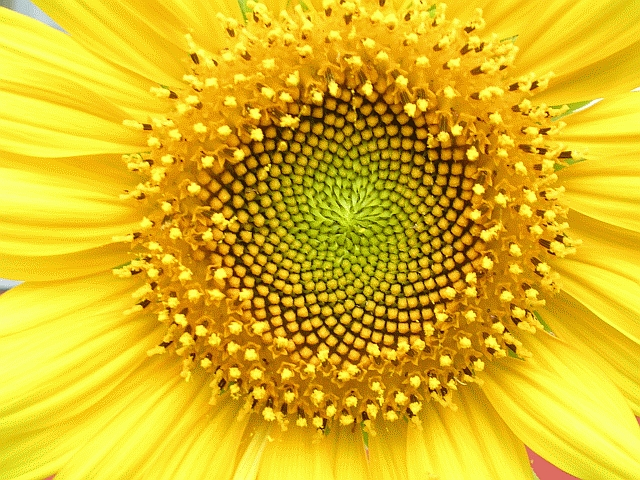
\includegraphics[height=2.7cm]{immagini-frazionarie/girasole.jpg} &
    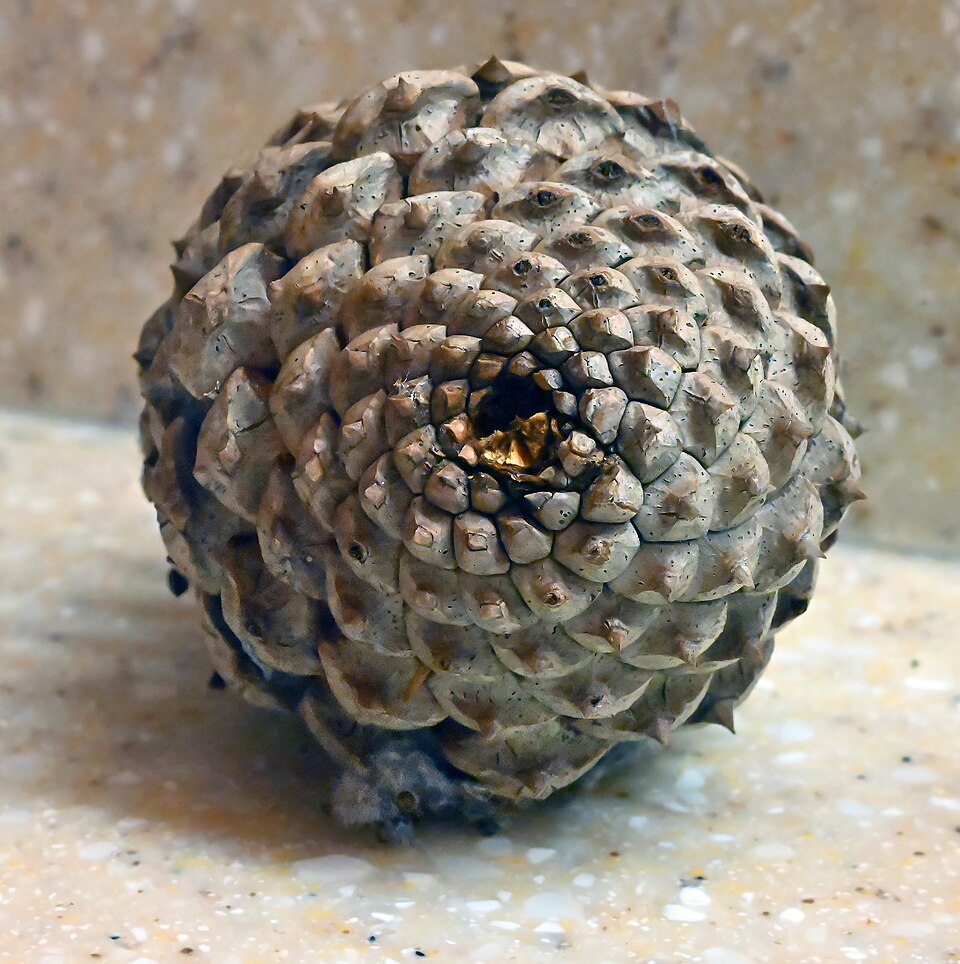
\includegraphics[height=2.7cm]{immagini-frazionarie/pigna.jpg} &
    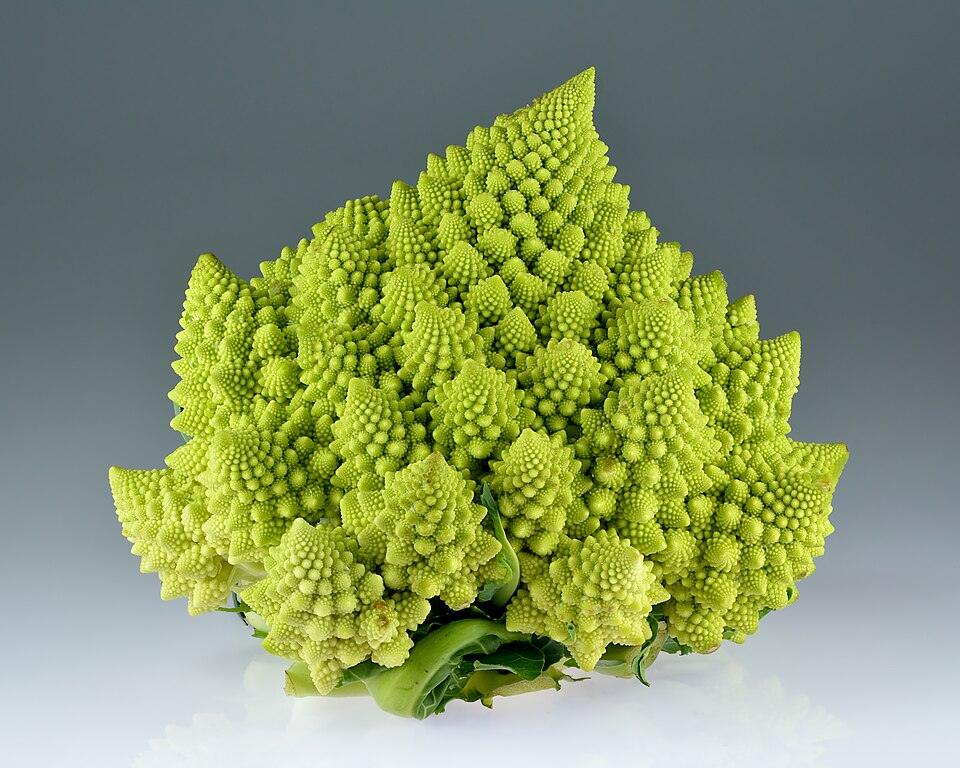
\includegraphics[height=2.7cm]{immagini-frazionarie/romanesco.jpg} &
    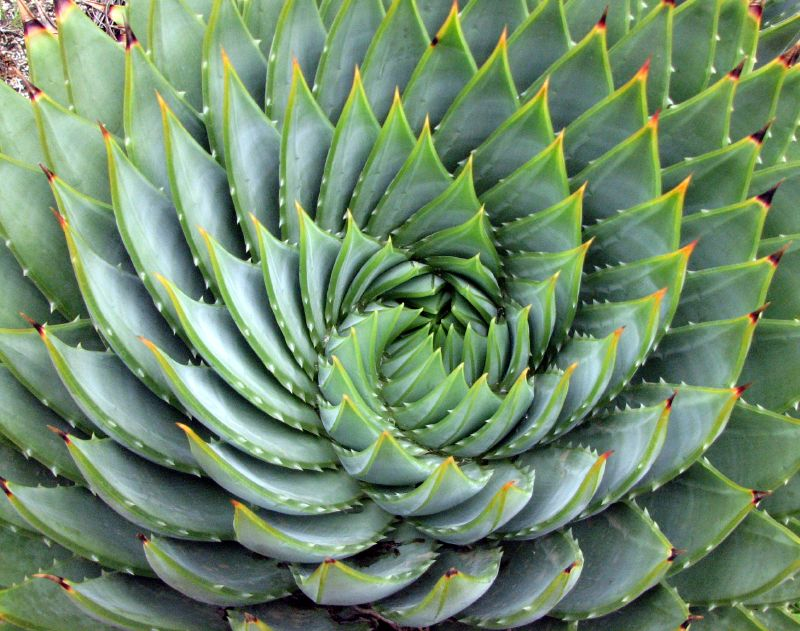
\includegraphics[height=2.7cm]{immagini-frazionarie/aloe.jpg} \\
    girasole & pigna & cavolo romanesco & \emph{Aloe polyphylla}
  \end{tabular}

  \vfill
  {\tiny\textcolor{grigio}{Immagini da Wikimedia Commons: girasole L.~Shyamal (CC BY-SA 2.5),
  pigna Bubba73 (CC BY-SA 4.0), romanesco Ivar Leidus (CC BY-SA 4.0), aloe Just chaos (CC BY 2.0).}}
\end{frame}

% ============================================================
% Metodo standard alla lavagna; le soluzioni compaiono in fondo.
\begin{frame}{Rifacciamo tutto con $x^2 = x$}
  \begin{columns}[T]
    \begin{column}{0.47\textwidth}
      \centering
      \textbf{Metodo standard}
      \[
        x^2 = x
      \]
    \end{column}
    \begin{column}{0.47\textwidth}
      \centering
      \textbf{Divido per $x$}
      \[
        x^2 = x
      \]
      \pause
      \[
        \frac{x^2}{x} = \frac{x}{x}
        \qquad\Rightarrow\qquad
        x = 1
      \]
    \end{column}
  \end{columns}
  \vfill
  \pause
  \begin{columns}[T]
    \begin{column}{0.47\textwidth}
      \centering $x = 0 \quad\vee\quad x = 1$
    \end{column}
    \begin{column}{0.47\textwidth}
      \centering $x = 1$ \quad \textcolor{rosso}{una sola soluzione!}
    \end{column}
  \end{columns}
  \pause
  \vspace{1.2em}
  \begin{center}
    \Large\textcolor{rosso}{Qual è l'errore?}
  \end{center}
\end{frame}

\begin{frame}{Non si può dividere per zero}
  \[
    x = 0: \qquad \frac{0^2}{0} = \frac{0}{0} \qquad \text{non ha senso}
  \]
  \pause
  \begin{alertblock}{}
    \centering Dividendo per $x$, che può valere $0$, si possono \textbf{perdere} soluzioni.
  \end{alertblock}
\end{frame}

\begin{frame}{E moltiplicando?}
  \[
    x - 1 = 0 \qquad\Rightarrow\qquad x = 1
  \]
  \pause
  Moltiplico sopra e sotto per $x - 2$:
  \[
    \frac{(x-2)(x-1)}{x-2} = 0
  \]
  \pause
  Una frazione vale zero quando il numeratore vale zero:
  \[
    (x-2)(x-1) = 0 \qquad\Rightarrow\qquad x = 1 \quad\vee\quad \textcolor{rosso}{x = 2}
  \]
  \pause
  \[
    x = 2: \qquad 2 - 1 = 0 \quad\Rightarrow\quad 1 = 0 \qquad \text{falso!}
  \]
  \pause
  \begin{alertblock}{}
    \centering Moltiplicando per $x-2$, che può valere $0$, si possono \textbf{guadagnare}
    soluzioni che non ci sono.
  \end{alertblock}
\end{frame}

\begin{frame}{Le equazioni frazionarie}
  \begin{block}{Definizione}
    Un'equazione si dice \textbf{frazionaria} quando l'incognita compare in almeno un denominatore.
  \end{block}
\end{frame}

\end{document}
